\chapter{Three-dimensional eddies structures}\label{Three-dimensional eddies structures}

In this chapter, we present statistical and descriptive results of the vertical structures of oceanic eddies from 2013 to 2018 from the SOSE model dataset. Vortex penetration depth, radius distribution in each layer, and different patterns of cyclonic and anticyclonic eddies are discussed here.

\section{Introduction}

Although a lot of studies focusing on surface altimetry have investigated the horizontal properties of the oceanic eddies, very few of them can answer the questions of what the vertical profile of the eddies looks like and how they will affect the estimate of the volume transport. What is worst, some of the previous studies put forward prior assumptions about the vertical shape of the eddies and the mathematics-derived result may not be so robust. Some researchers want to deduce the vertical structure from Argo float data. However, time lag between the time when a float reaches the surface and the time when it reports its location with the Argos positioning satellite, and positioning errors limited by the accuracy of the Argos positioning system may raise the uncertainty of the identification\cite{chaigneau2011vertical}.

Most of the past research or publications only focus on the two-dimensional plot of oceanic eddies, partly because only the ocean surface observations are available, and partly because the magnitude of vertical velocity is three-orders less than the horizontal velocity, yielding a lot of noise to produce three-dimensional analysis and construct the three-dimensional structure. Sparse distribution of the observational array can only capture a limited picture of eddies features and thus ocean model, which provides a three-dimensional panoramic view of the ocean, fills in the gap in our understanding of three-dimensional ocean state variable 

One feasible solution is using Lagrangian tools such as drifts or Argo floats, with the hope that drifts are located around the eddy cores and the selected interpolation scheme is suitable to estimate the real oceanic state around the eddies.

Questions still exist about the three-dimensional structure of oceanic eddies: (1) how do the eddies extend in the vertical direction; (2) how do eddies enhance the stirring and coupling of the upper ocean and deep ocean.

There is great concern about the understanding gap between the surface eddies and deep eddies. The ocean is divided into three zones in the vertical direction: a well-mixed surface region, rapidly varying ocean subsurface thermocline, and the stratified ocean interior. The ocean surface and ocean interior, with distinct features and separated by the thermocline, set up the questions about the relationship between surface eddies and deep eddies. Some eddies are constrained only to the surface, some will extend to the deep sea, while others subsurface eddies show no sign of the surface height signal. Worse still, it is rather difficult to extract Lagrangian
structures and elaborate their effect on mixing properties in unsteady 3-D flow due to the explosion of complexity \cite{aref2017frontiers}.  

\section{3D structure construction algorithms for an eddy}

In chapter \ref{Lagrangian eddies detection}, we show how to set up a computational process and detect eddy on the surface. Repeating the same process and using the flow field information at 42 layers in the numerical data, we could get the 3D structure of coherent eddy. As discussed in the previous paper, an eddy center would not drift by 1/4
of its radius when it goes down 50 m if it is still detectable \cite{dong2012three}.

Thus, the overall workflow of the detection would be as follows:

\begin{itemize}
  \item [1)] 
  Compute the LAVD field in each depth layer and extract eddies from the surface layer to the other below layers following the same process in Chapter \ref{data and methodology}.
  \item [2)]
  Group the extracted eddies according to their characteristics and then  select eddies based on judging criteria ``an eddy center would not drift by 1/4 of its radius when it goes down 50 m".
  \item [3)]
  If in the same depth level, more than one eddies were found, pick the vortex with the closest horizontal distance from the surface one.
\end{itemize}


\section{Eddies penetration depth and three-dimensional shape type}

To construct the vertical profile of the eddies, we use the velocity filed results generated from SOSE oceanic model. The horizontal resolution of SOSE dataset is $ \frac{1}{6}^{\circ} $ and SOSE dataset has 41 layers in the vertical direction in total, covering variables from the surface to 5km in depth.

We have detected 732 eddies in the surface layer from 2013 to 2018 and 566 ($77\%$) of them were found to have signals in the below layers and  used to construct the 3-D structure in the research, which suggests an amount of about $25\%$ of the eddies is quite shallow

From figure \ref{Depth Frequency.png}, we could find that about half of the eddies could still be detected at a depth of 2010 meters, about $20\%$ of the eddies have depths ranging from 1500 m to 1800 m, and about $18\%$ of them reach the depth of 1000m to 1500 m.

\begin{figure}[htbp]
    \centering
    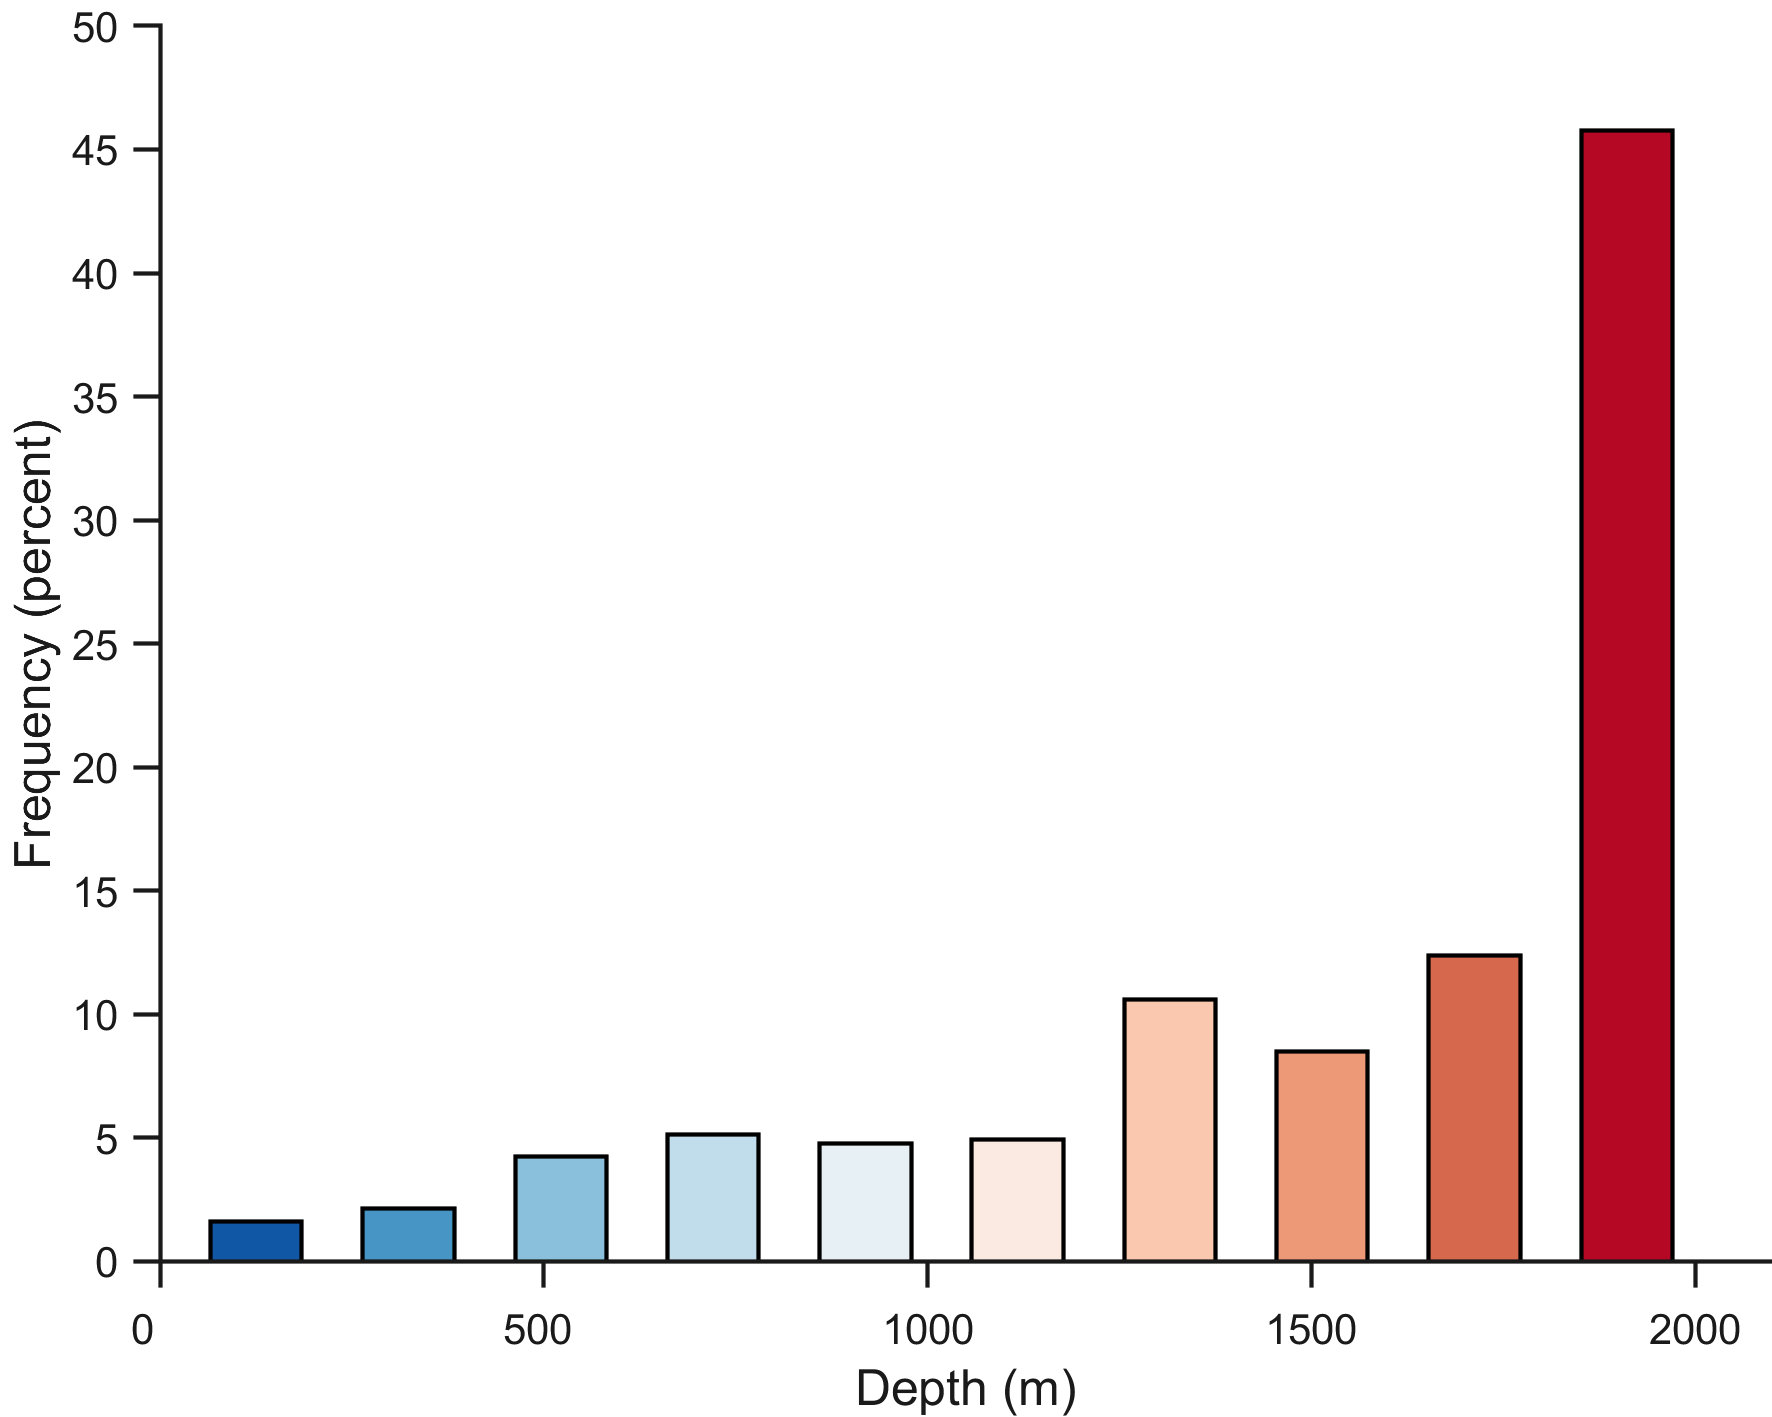
\includegraphics[width =12cm]{chapter/figure/Depth Frequency.png}
    \caption{Histogram distribution map of vortex depth}
    \label{Depth Frequency.png}
\end{figure}

Among all the 566 3-D eddies, about $52\%$ of them (294) are cyclonic eddies and about $48\%$ of them are anticyclonic ones. The maximum vortex radius of the cyclonic eddies is placed at depth of around 826 meters while the maximum vortex radius of the anticyclonic eddies centers at depth of 659 meters or so. The average value of the maximum depth of the cyclonic vortices is about 1679 meters and the mean value of the maximum depth of the depth extension of anticyclonic eddies is 1496 meters. The above findings show us that cyclonic eddies tend to have a greater vertical extension and thus they have stronger transport capacity and could carry more volume of seawater.

According to existing papers, the eddy vertical shape of oceanic eddies could be classified into three kinds: eddies with the largest semidiameter on the surface like a bowl, cone-shaped vortices with the largest radius at the bottom layer, and lens-shaped eddies having the largest size in the middle \cite{dong2012three,lin2015three}.

In the Argentine basin, all those three types of eddies were found and lens-shaped eddies are the majority:  72 of the detected eddies were bowl-shaped, 412 of them are lens-shaped and 82 of the eddies are cone-shaped vortices. The following figures from \ref{bowl-shaped.png} to \ref{cone-shaped.png} show the vertical distribution of some selected eddies. Figure \ref{bowl-shaped.png} illustrates three bowl-shaped eddies having a maximum radius on the surface and then decreasing towards the bottom. Figure \ref{lens-shaped.png} shows three eddies having maximum radius in the intermediate layer and then becoming smaller with increasing depth. In figure \ref{cone-shaped.png}, eddies on the surface are the smallest, gradually get larger, and reach a maximum at the bottom. The vortex radius may be more stable in size in the intermediate layer.

\begin{figure}[htbp]
    \centering
    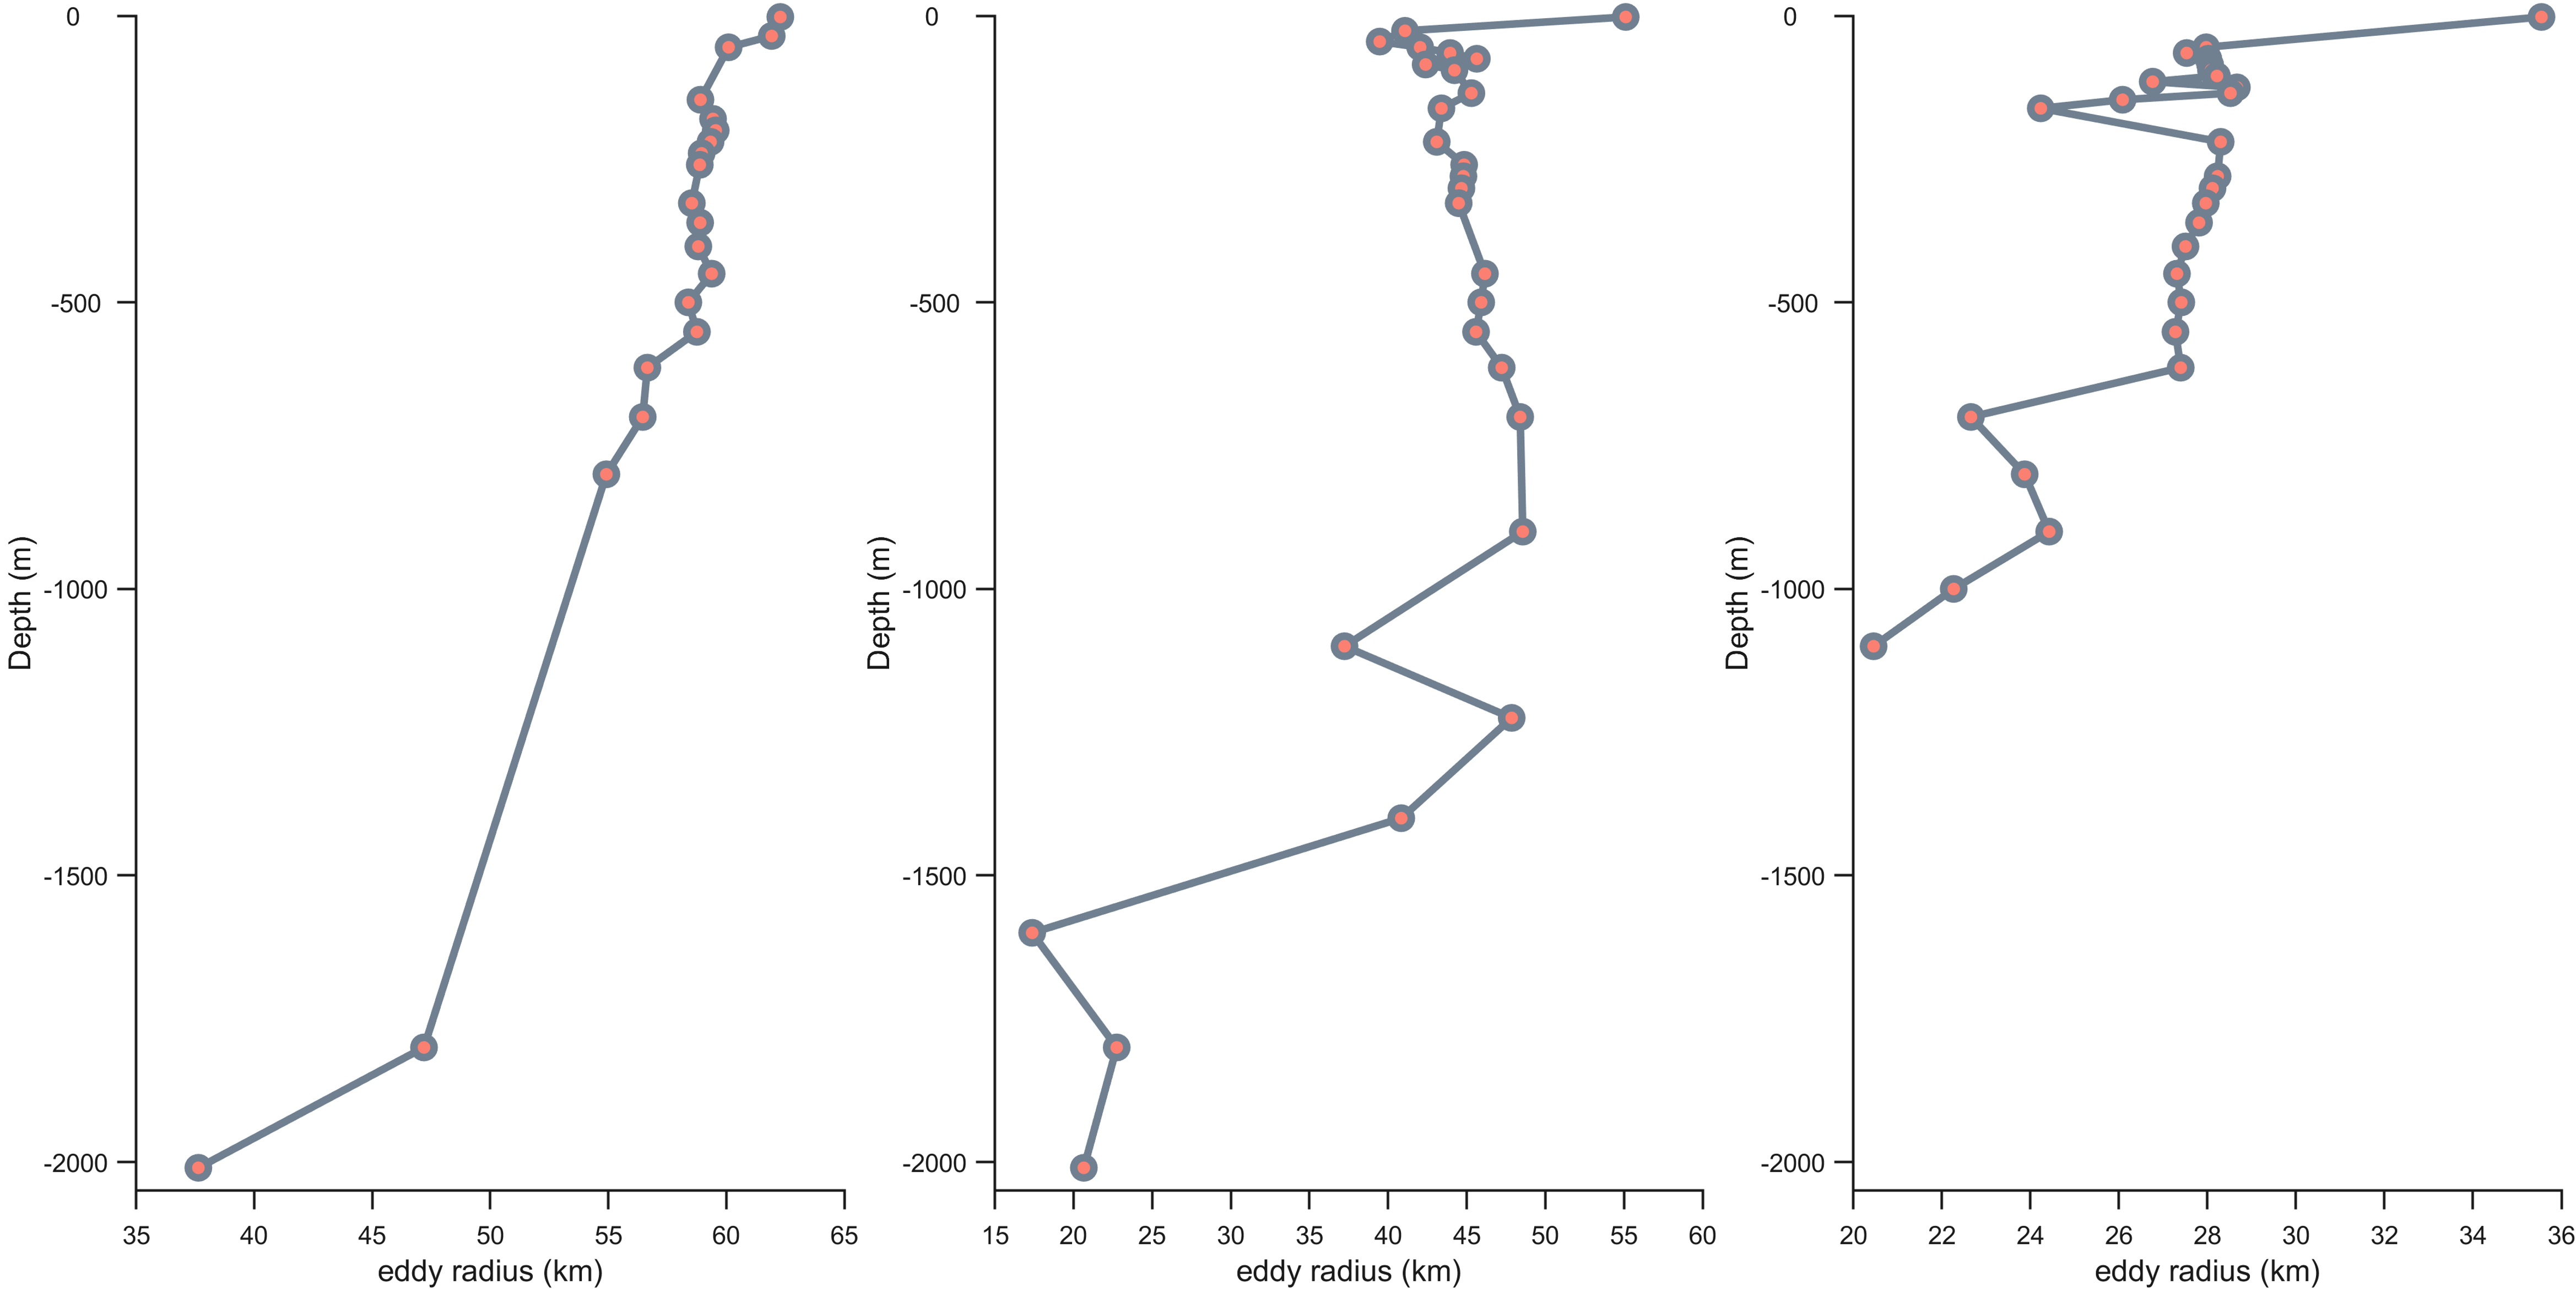
\includegraphics[width=1.0\textwidth]{chapter/figure/bowl-shaped.png}
    \caption{Three examples of bowl-shaped eddies}
    \label{bowl-shaped.png}
\end{figure}

\begin{figure}[htbp]
    \centering
    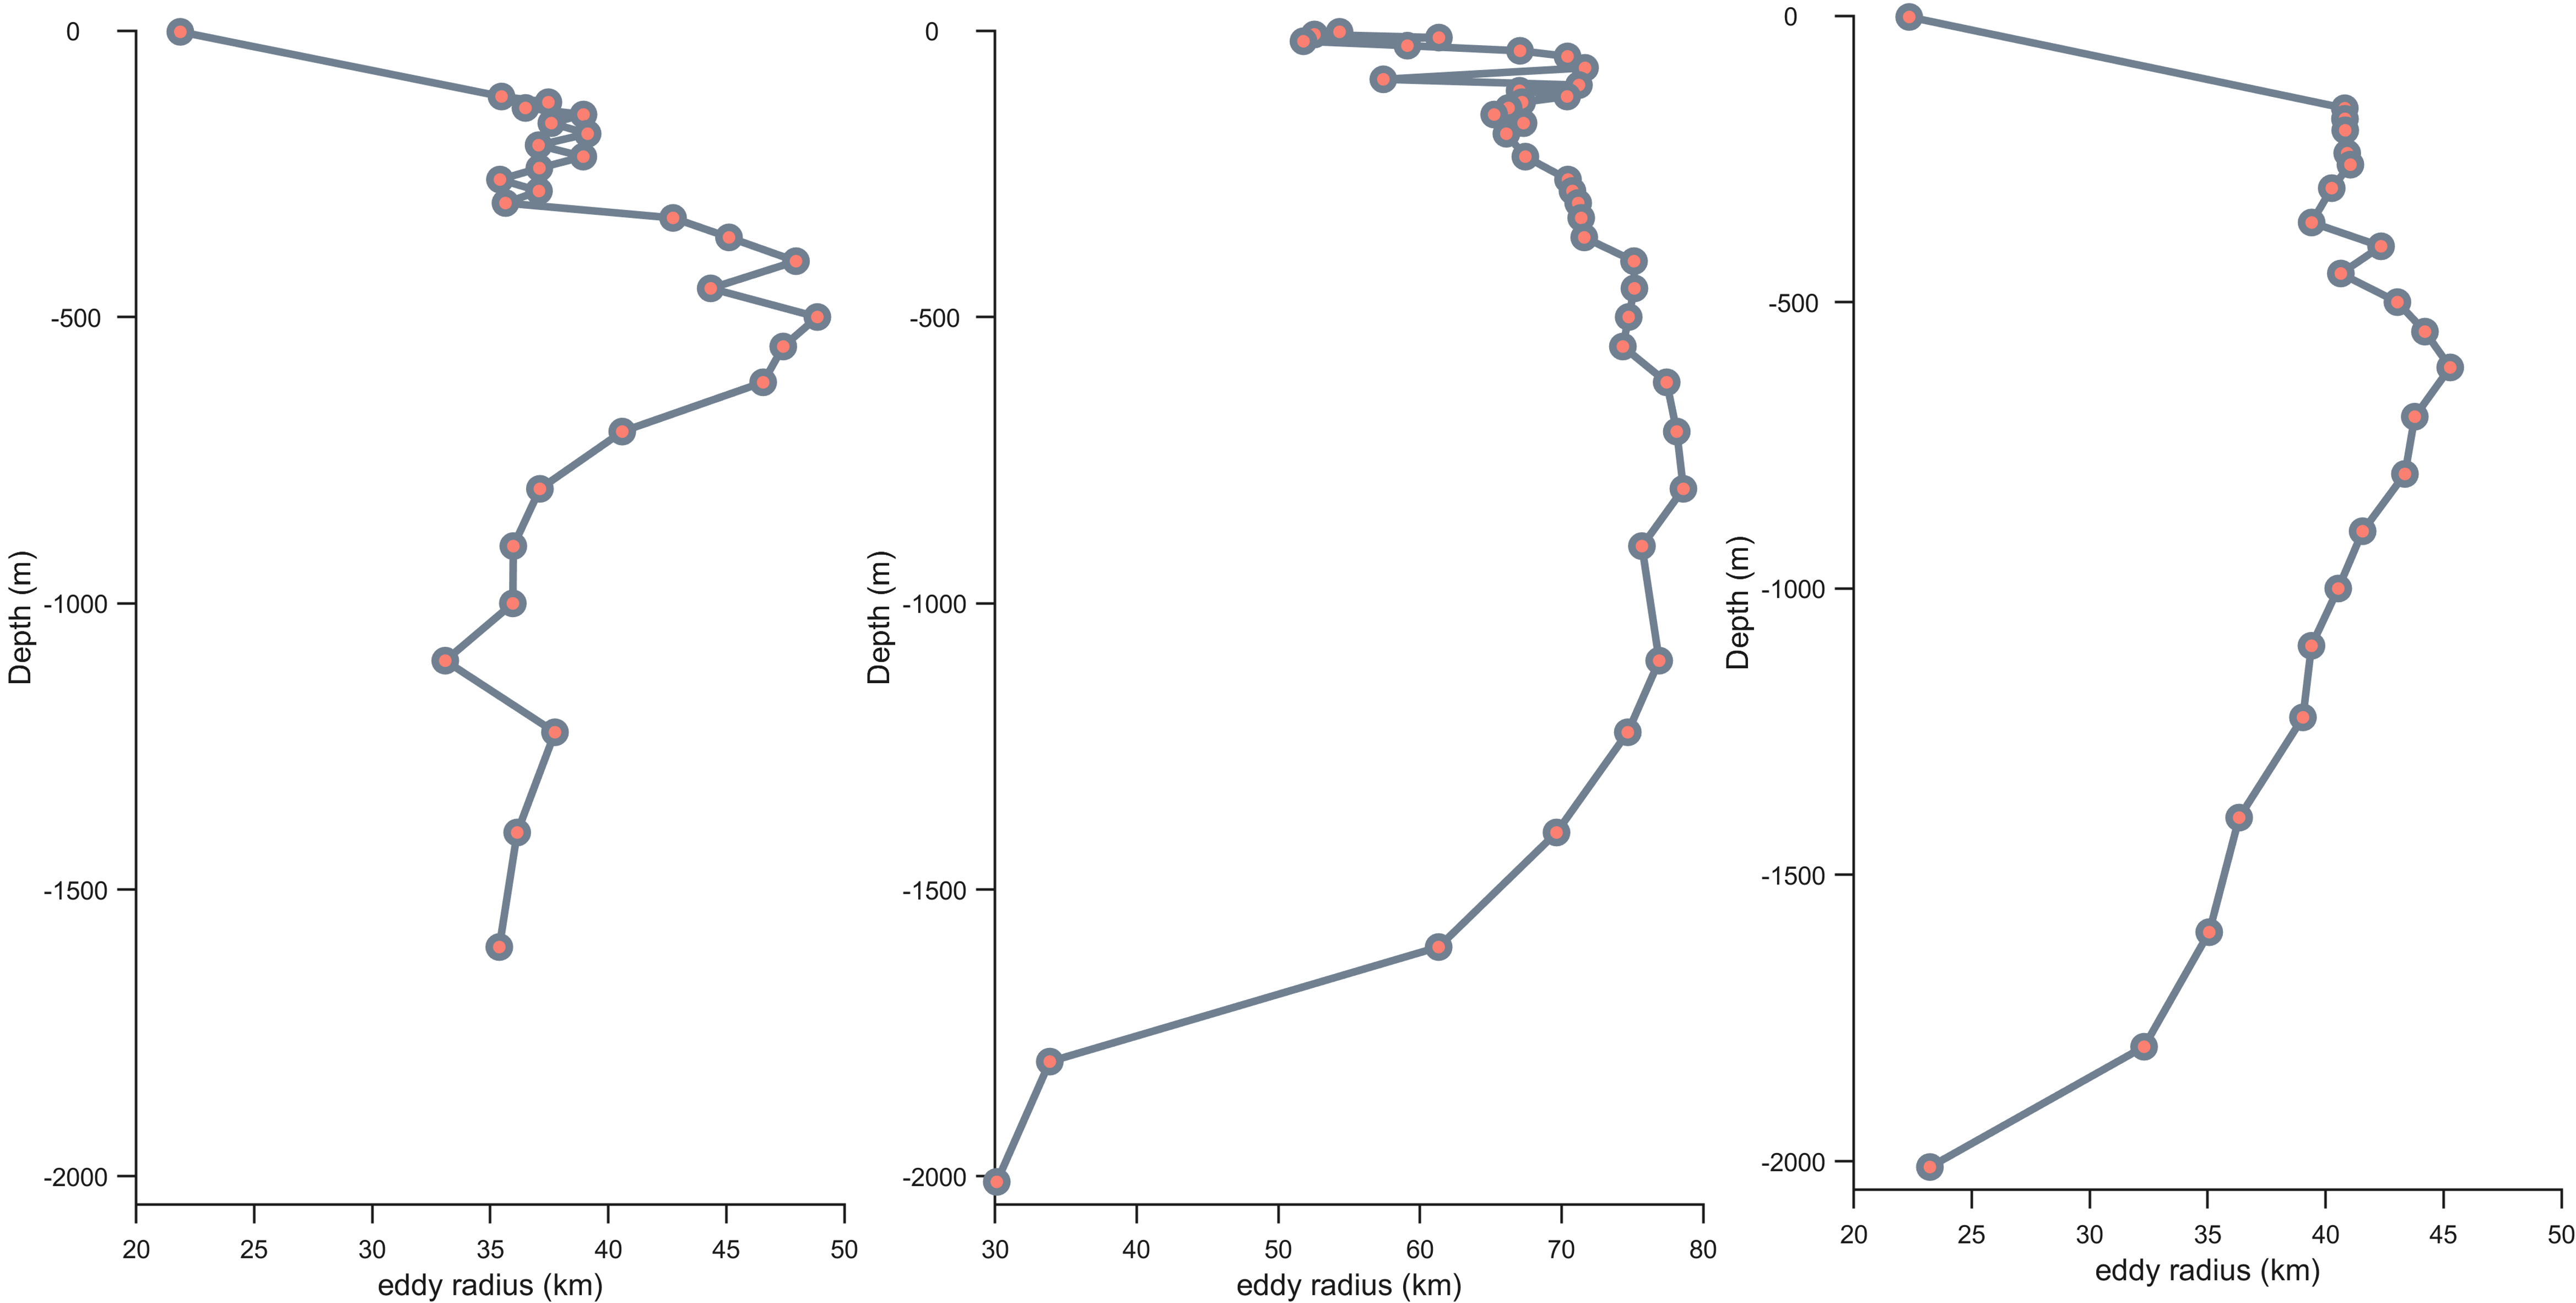
\includegraphics[width = 15cm]{chapter/figure/lens-shaped.png}
    \caption{Three examples of lens-shaped eddies }
    \label{lens-shaped.png}
\end{figure}

\begin{figure}[htbp]
    \centering
    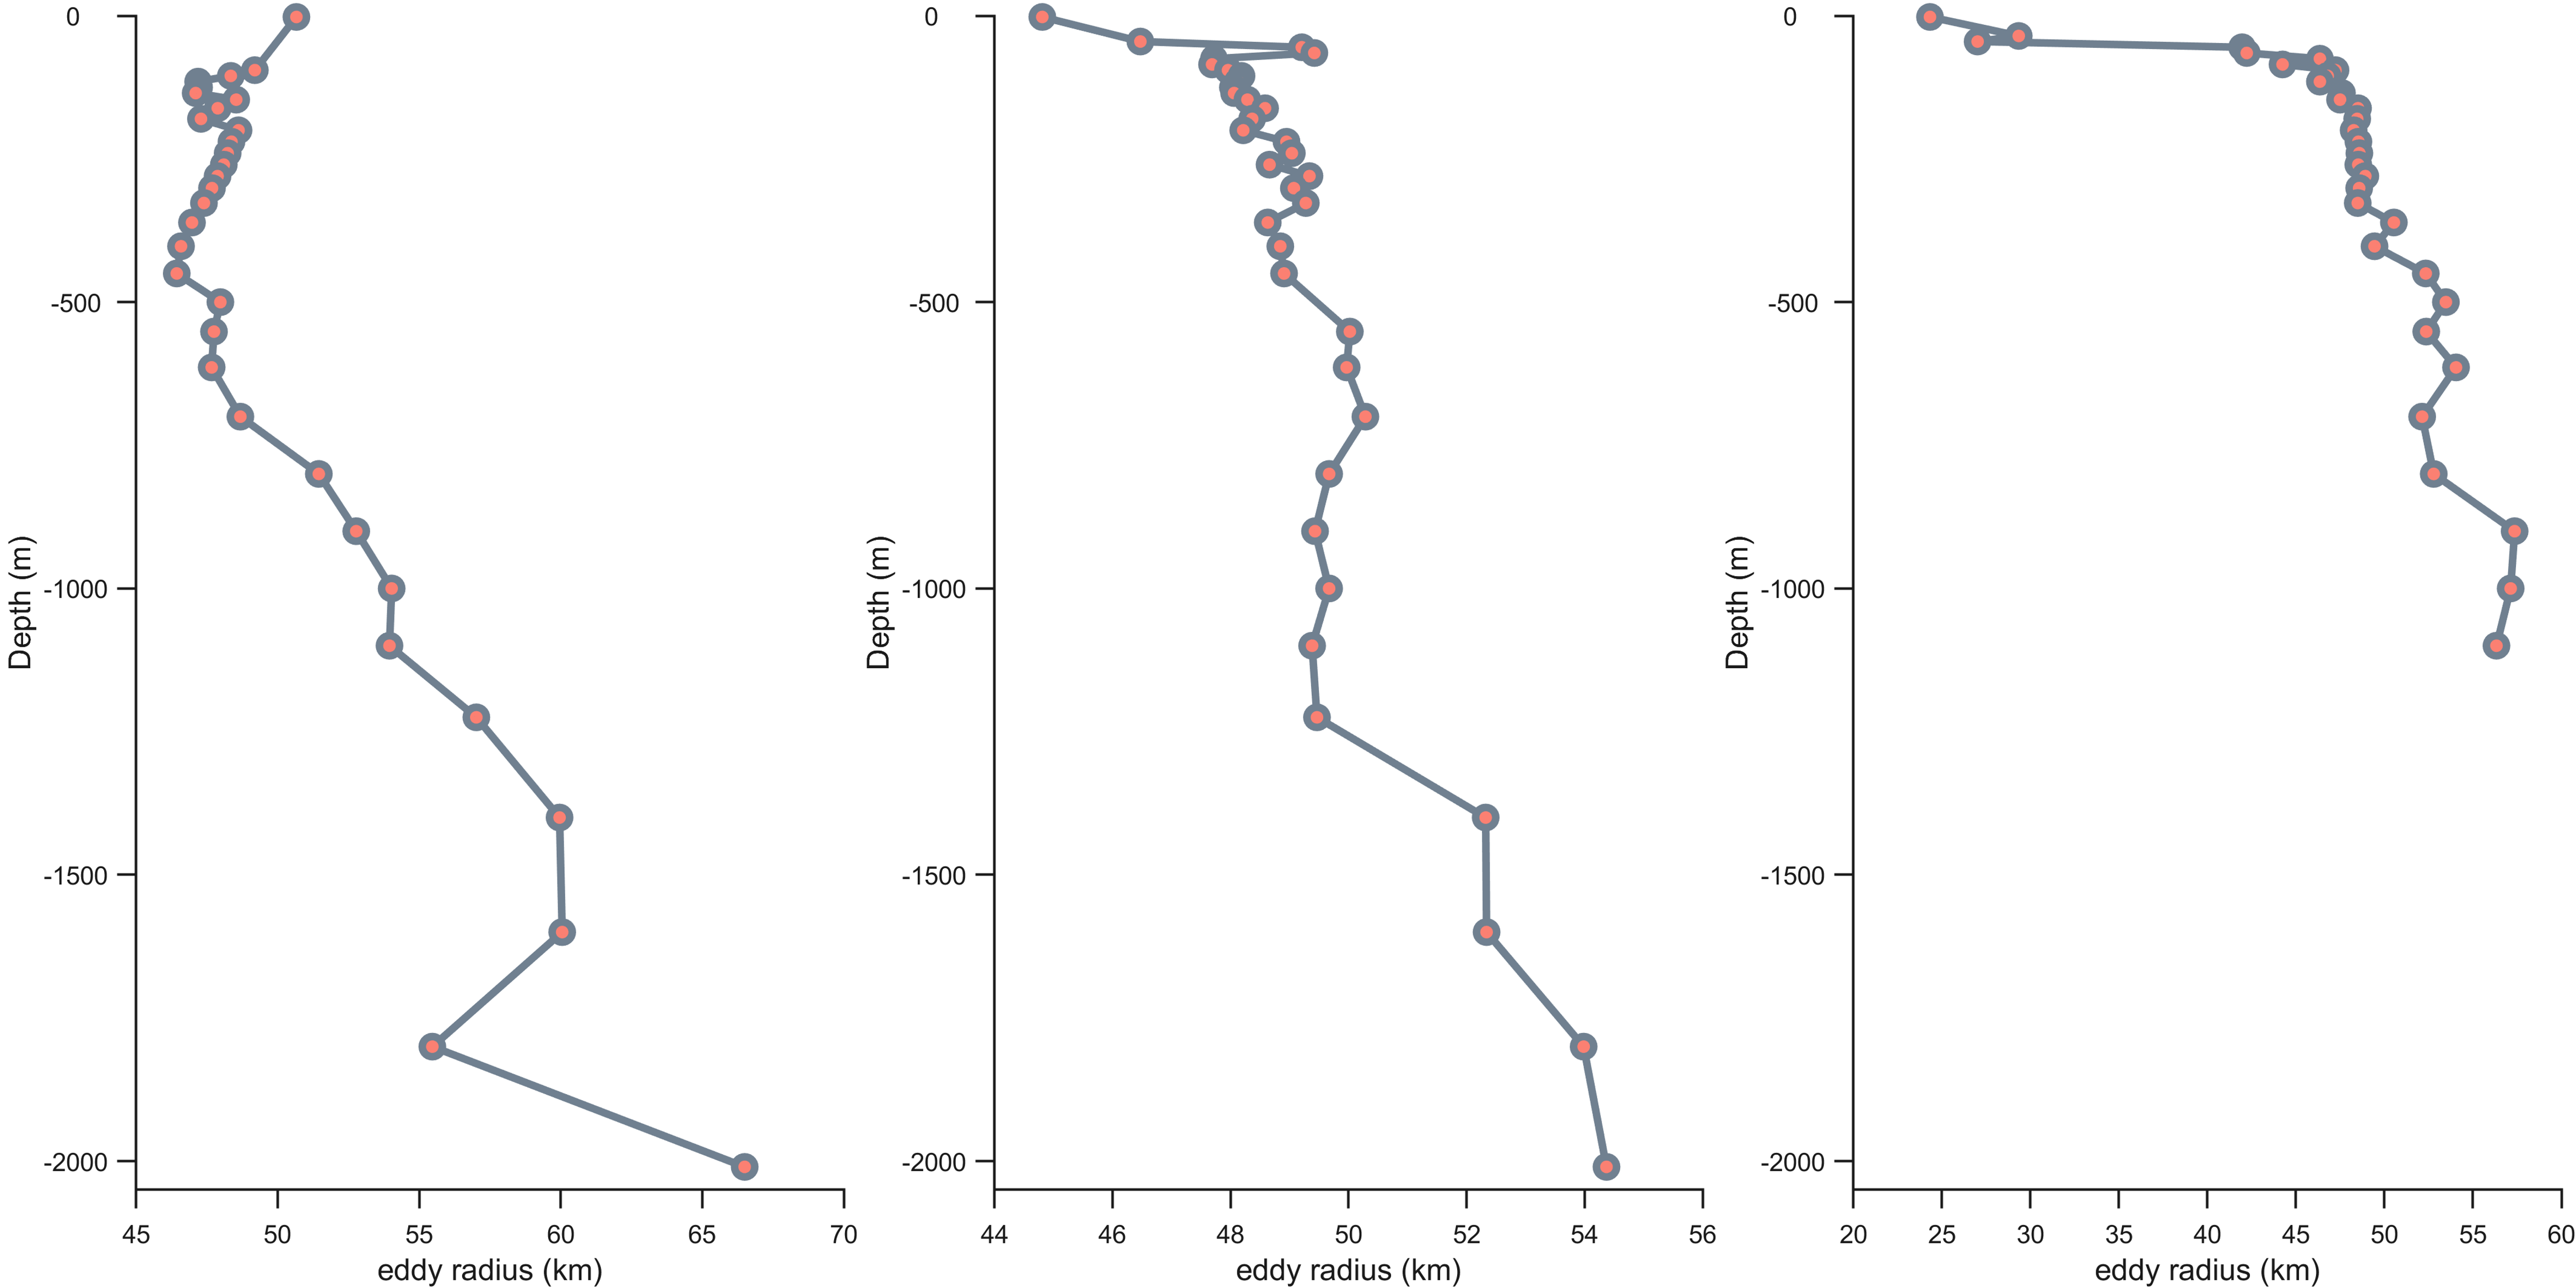
\includegraphics[width = 15cm]{chapter/figure/cone-shaped.png}
    \caption{Three examples of cone-shaped eddies}
    \label{cone-shaped.png}
\end{figure}





\section{Case studies of oceanic eddies}

Figure \ref{cyclonic-3D.png} shows the vertical slice of salinity field and radius distribution of a cyclonic coherent eddy with $t_0 = 2014-01-01$. We could find that the subsurface vortex radius has a maximum value of and the eddy's size changes dramatically on the surface. In section (a) of the figure \ref{cyclonic-3D.png}, each slice represents the salinity distribution in each depth layer. The minimum value of the salinity is at the blue end of the color chart while the maximum value of the regional salinity is represented by the red color of the color chart; the color bar shown on the left side  only displays the salinity limit on the bottom layer. The surface eddy is the center of the negative anomalous envelope of salinity and in the below layers, the eddy is surrounded by high salinity contour. These findings suggest that cold and salty coherent cyclonic eddy may upwell the bottom water column into the subsurface layers. 

Figure \ref{2014-12-24_6.png} shows an anticyclonic eddy with maximum radius in the intermediate layer and $t_0 = 2014-12-01$. It has a warm core of the water in the center of the eddy. However, the area of the high-temperature contour is much bigger than the area enclosed by the eddy, which we could infer that coherent water transport capabilities carried by the coherent eddy may be much weaker than what we have expected in an Eulerian instantaneous field.  

However, in some of the cases, the extreme value of the background salinity ($S$) or temperature ($\theta$) field does not match the core of the coherent eddies. In some of the cases, the background extrema of $S$ or $\theta$ may shift a little bit from the eddy center. This asymmetry feature is more obvious in the vertical structure of anticyclonic eddies \cite{sandalyuk2021three}.

What is more, the above rules are not so robust in the surface layer, especially the first 100 meters, which suggests the other boundary layer mixing processes can significantly affect the character of the vortex.


\begin{figure}[htbp]
    \centering
    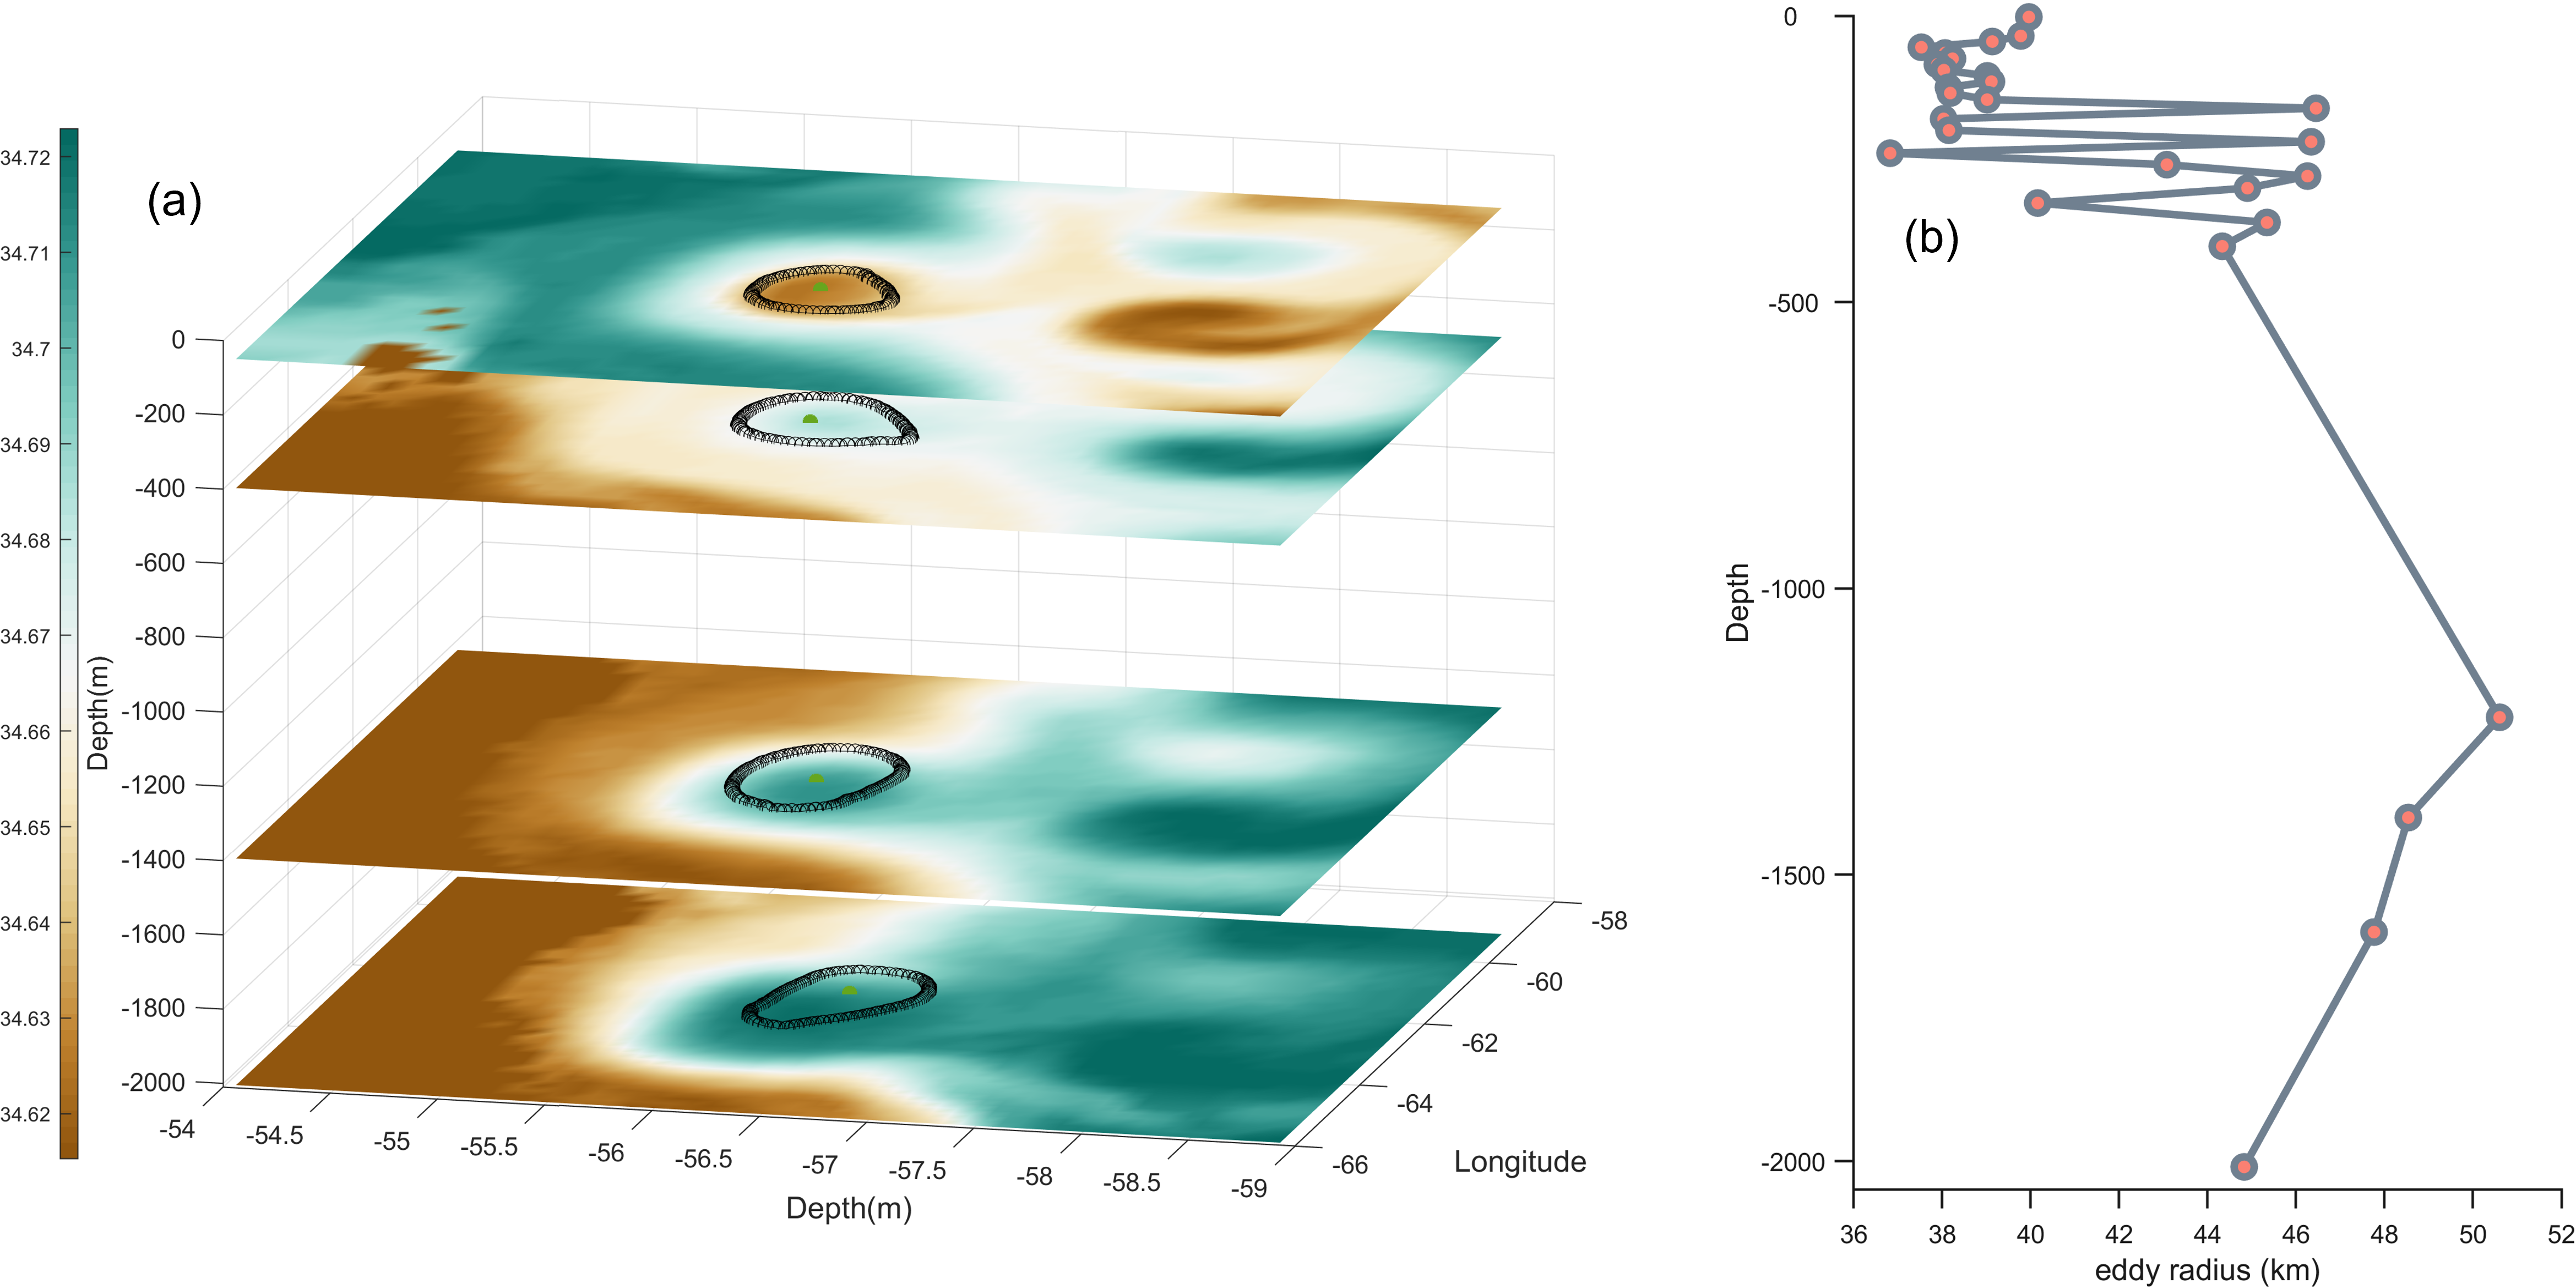
\includegraphics[width = 1\textwidth]{chapter/figure/cyclonic-3D.png}
    \caption{Vertical structure of a cyclonic eddy}
    \label{cyclonic-3D.png}
\end{figure}

\begin{figure}[htbp]
    \centering
    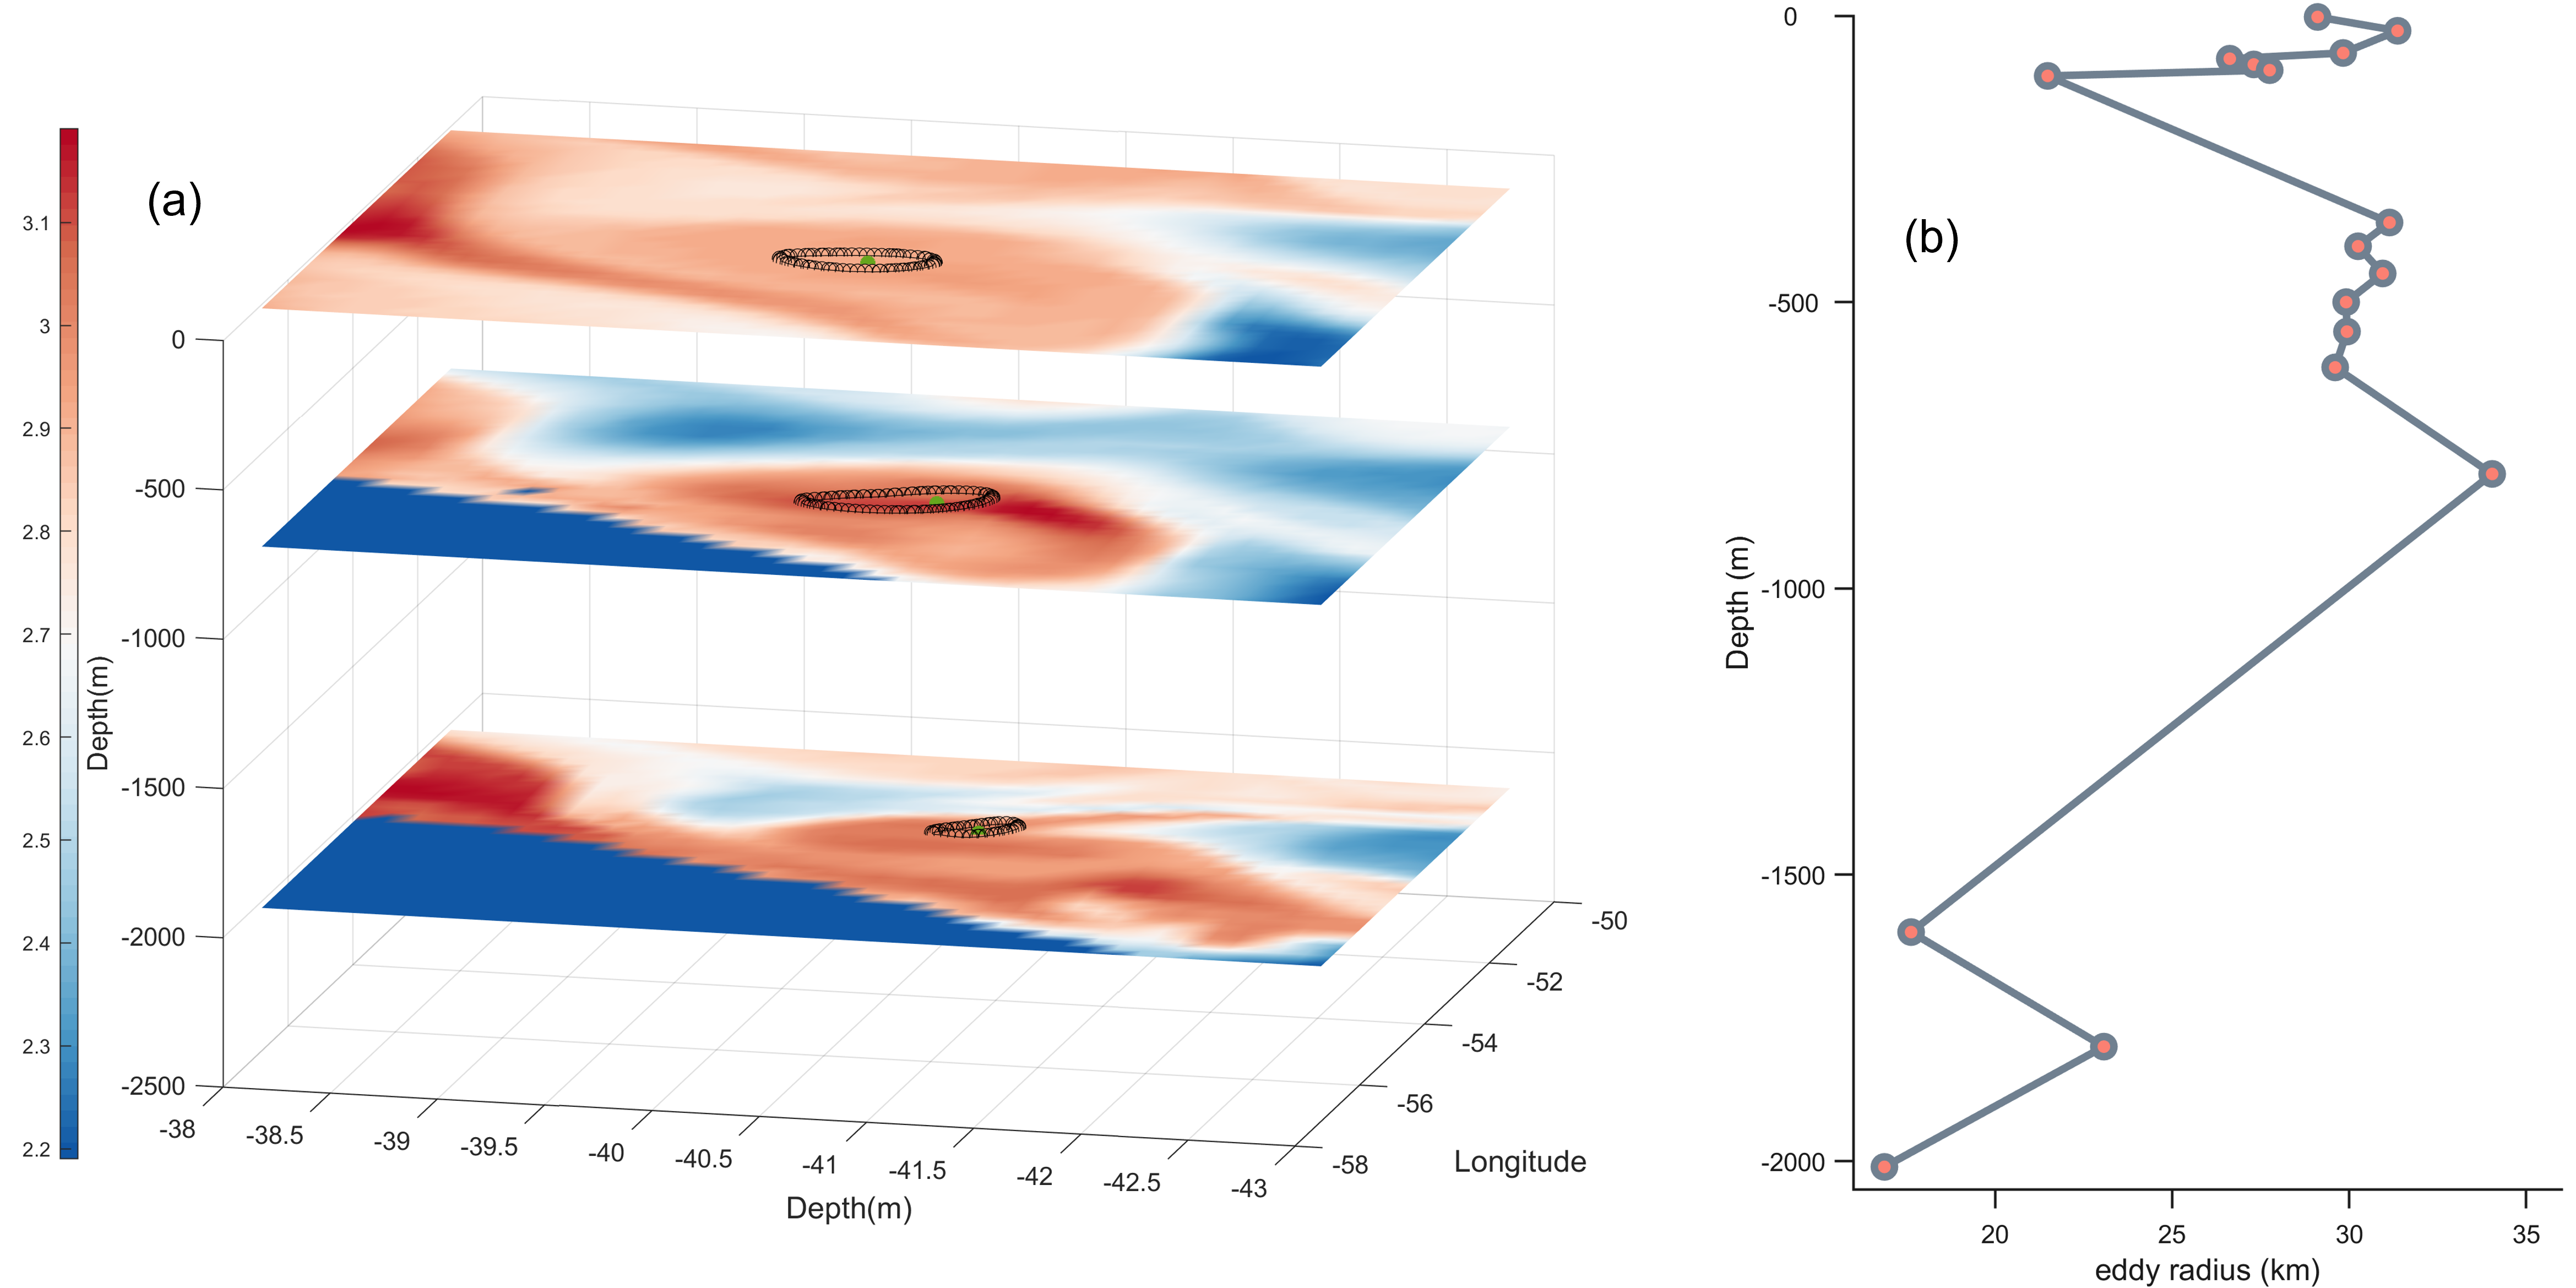
\includegraphics[width = 1\textwidth]{chapter/figure/2014-12-24_6.png}
    \caption{Vertical structure of an anticyclonic eddy}
    \label{2014-12-24_6.png}
\end{figure}

\clearpage

\section{Discussion and Conclusion}

Due to the limiting subsurface observational data, we build the three-dimensional structure of coherent eddies using model simulations. 

It is still questionable if we do capture the correct shape and penetration depth of coherent eddies and the visualization of propagation of three-dimensional eddies in the real oceanic flow is still on the way \cite{liu2018gulf}. We track surface eddies in this chapter and we attempt to trace the corresponding vortex signal in the subsurface. 

We have found three types of eddies in the study period (2013-2018), most of them are ens-shaped eddies having a maximum radius in the intermediate layer. Cyclonic eddies have the tendency to extend in the vertical direction. Eddies could alter the thermohaline properties of seawater: the cyclonic vortex is colder and saltier than the surrounding water column while the anticyclonic eddy is warmer and fresher.


\newpage
